% ============================================================
%  深圳大学实验报告模板（SZU Experiment Report Template）
% This template can be modified according to the specific requirements of your experiment or project.
% Produced by: Chao Fan and Kewei Ou, AI School of SZU
% ============================================================

\documentclass[a4paper,12pt]{article}

% ----------------------------
% 中文与字体支持
% ----------------------------
\usepackage{fontspec}    % 字体支持
\usepackage{xeCJK}       % 中文字体支持
\setCJKmainfont{FandolSong-Regular} % TeX Live / Overleaf 均可用的中文字体
\setCJKmonofont{FandolSong-Regular}
\usepackage{indentfirst}
\setlength{\parindent}{2em}
\usepackage[hidelinks]{hyperref}
% ----------------------------
% 页面设置与常用宏包
% ----------------------------
\usepackage{geometry}    % 页面边距控制
\geometry{left=1in, right=1in, top=1in, bottom=1in}

\usepackage{longtable}   % 支持长表格
\usepackage{booktabs}    % 三线表
\usepackage{amsmath}     % 数学公式
\usepackage{array}       % 表格列格式
\usepackage{graphicx}    % 插入图片
\usepackage{fancyhdr}    % 页眉页脚控制
\usepackage{tikz}        % 绘制框线等图形
\usetikzlibrary{calc,positioning} % 坐标计算与相对定位
\usepackage{verbatim}    % 显示代码块
\usepackage{float}       % 控制图片浮动位置（[H]参数）
\usepackage{xcolor}      % 红色标注个人贡献与可复现性信息
\newcommand{\studenthighlight}[1]{\textcolor{red}{\textbf{#1}}}

% ----------------------------
% 页眉页脚设置
% ----------------------------
% \pagestyle{fancy}
\fancyhf{} % 清空默认页眉页脚
% \fancyhead[L]{深圳大学实验报告} % 左侧页眉文字
\fancyhead[C]{} % 中间空
\fancyhead[R]{} % 右侧空

% ============================================================
%                      文档开始
% ============================================================

\begin{document}

% ============================================================
% 封面页
% ============================================================
\begin{titlepage}
    \centering
    \vspace*{2cm}
    \Huge{\textbf{深 \ 圳 \ 大 \ 学 \ 实 \ 验  \ 报 \ 告}}\\[1.5cm]
    
    {\Large\textbf{课程名称}\quad\underline{\makebox[8cm][c]{Python程序设计}}}\\[0.5cm]
{\Large
\noindent\makebox[3.2cm][l]{\textbf{项目名称}}
\underline{\makebox[8cm][c]{复现OpenCLIP ViT-B-32图像编码器}}}\\[0.5cm]
{\Large
\noindent\makebox[3.2cm][l]{\textbf{学 \quad \quad 院}}
\underline{\makebox[8cm][c]{人工智能学院}}}\\[0.5cm]
{\Large
\noindent\makebox[3.2cm][l]{\textbf{专 \quad \quad 业}}
\underline{\makebox[8cm][c]{人工智能专业}}}\\[0.5cm]
{\Large
\noindent\makebox[3.2cm][l]{\textbf{指导教师}}
\underline{\makebox[8cm][c]{樊超}}}\\[0.5cm]
{\Large
\noindent\makebox[3.2cm][l]{\textbf{报 \quad 告 \quad 人}}
\underline{\makebox[3cm][c]{蔡若欣}}
\hspace{0.5cm}
\textbf{学号}
\underline{\makebox[3cm][c]{2025681069}}}\\[0.5cm]
{\Large
\noindent\makebox[3.2cm][l]{\textbf{实验时间}}
\underline{\makebox[8cm][c]{2026年11月3日-11月22日}}}\\[0.5cm]
{\Large
\noindent\makebox[3.2cm][l]{\textbf{提交时间}}
\underline{\makebox[8cm][c]{2026年11月18日}}}\\[1.5cm]

    \vfill
    \Large{\textbf{教务处制}}
\end{titlepage}

\newpage

% ============================================================
% 正文部分
% ============================================================
\section{实验目的}

本实验使用NumPy复现OpenCLIP ViT-B-32的图像编码器前向计算。输入为经过给定预处理的\texttt{float32}图像批次，形状为 $[B,3,224,224]$；输出为每张图像对应的512维单位向量，要求与课程提供的独立FP32参考结果在给定容差内逐项一致。\studenthighlight{本人实现的工作为模型前向计算，不包含训练、反向传播或参数更新。}检查点中的152个视觉张量在整个前向过程中保持固定。


实验的具体目标：
\begin{enumerate}
    \item \studenthighlight{按给定接口规范完成图块划分、注意力头拆分与合并、Transformer block、嵌入与最终输出六组实现；}
    \item \studenthighlight{通过逐阶段误差比对确认NumPy实现与参考实现等价；}
    \item \studenthighlight{在检查点权重布局与课程约定不一致的部位（线性层权重的存储方向）建立正确的前向计算，避免出现形状不匹配或数值系统性偏移。}
\end{enumerate}

\section{实验环境与数据}

实验在 Windows 环境下使用 Python 3.9 及以上版本执行，核心依赖为 NumPy 和 Pillow；模型前向计算仅使用 CPU，不使用 PyTorch、OpenCLIP 包、GPU 或网络下载。课程附件提供固定配置、10 张本地图像、152 个视觉参数张量及独立 FP32 参考输出。实现和验证所使用的关键对象如下：

\begin{table}[H]
\centering
\small
\caption{实验输入与模型固定配置}
\label{tab:environment}
\begin{tabular}{l l}
\toprule
项目 & 内容 \\
\midrule
输入图像 & 已预处理的 \texttt{float32} 数组，形状为 $[B,3,224,224]$ \\
图块配置 & 图块边长 $32$，网格为 $7\times7$，共 49 个图块 \\
视觉编码器 & ViT-B-32，宽度 $768$，12 个 Transformer block，12 个注意力头 \\
MLP 中间维度 & $3072$ \\
输出 token & 归一化 \texttt{float32} 数组，形状为 $[B,512]$ \\
验证数据 & \texttt{assets/reference\_outputs.npz}，含中间阶段与最终输出 \\
\bottomrule
\end{tabular}
\end{table}

\section{实验原理与总体流程}

模型首先将图像划分为 $7\times7=49$ 个 $32\times32$ 的 RGB 图块。每个图块按 C--H--W 顺序拉平成 3072 维向量，再投影为 768 维 token。随后在 token 序列首部拼接 CLS token，并叠加 50 个学习得到的位置向量。12 个 Transformer block 对序列进行编码，每个 block 的宽度 D=768，包含 12 个注意力头、每个头 64 维，MLP 的中间维度为 3072。编码结束后仅取序列第 0 行的 CLS token，经过后置 LayerNorm、$768\rightarrow512$ 的线性投影与 $L_2$ 归一化，得到每张图像的输出向量。整体流程如图\ref{fig:overall-flow}所示。

\begin{figure}[H]
\centering
\begin{tikzpicture}[node distance=5mm and 5mm, every node/.style={draw, align=center, minimum height=9mm, font=\small}]
\node (img) {输入图像\\$[B,3,224,224]$};
\node [right=of img] (patch) {Patchify\\$[B,49,3072]$};
\node [right=of patch] (embed) {线性投影 + CLS + 位置\\$[B,50,768]$};
\node [below=of embed] (trans) {12 个 Transformer blocks\\$[B,50,768]$};
\node [left=of trans] (out) {CLS + PostNorm + Proj + $L_2$\\$[B,512]$};
\draw[->,thick] (img) -- (patch);
\draw[->,thick] (patch) -- (embed);
\draw[->,thick] (embed) -- (trans);
\draw[->,thick] (trans) -- (out);
\end{tikzpicture}
\caption{图像编码器的端到端张量流程}
\label{fig:overall-flow}
\end{figure}

整个前向过程按以下五步执行。每一步均保持 \texttt{float32} 精度，避免在多层矩阵乘法中因默认 \texttt{float64} 或不一致的广播规则产生额外误差。

\begin{enumerate}
    \item \textbf{读取与预处理：}将原始 RGB 图片按最短边缩放、中心裁剪为 $224\times224$，由 HWC 转为 CHW，并按给定均值和标准差标准化，得到 $[B,3,224,224]$。
    \item \textbf{图块构造：}按行优先遍历 $7\times7$ 网格，每个图块保留 C--H--W 内部顺序，输出 $[B,49,3072]$。
    \item \textbf{输入 token 组装：}图块通过线性投影变为 768 维，在首部拼接 CLS token，再与 50 行位置嵌入逐元素相加，得到 $[B,50,768]$。
    \item \textbf{Transformer 编码：}连续执行 12 个 ``LayerNorm--多头注意力--残差--LayerNorm--MLP--残差'' block，token 数和隐藏宽度保持不变。
    \item \textbf{最终输出与验证：}选取第 0 行 CLS token，执行后置归一化和 $768\rightarrow512$ 投影，最后进行 $L_2$ 归一化；再与每个参考阶段逐元素比较。
\end{enumerate}

\section{实现说明}



\subsection{图块与嵌入}

\studenthighlight{\texttt{patchify}} 使用 \texttt{reshape} 与 \texttt{transpose} 两个操作完成形状变换，先将输入$[B,3,224,224]$重排为 $[B,3,7,32,7,32]$，再用 \texttt{transpose(0,2,4,1,3,5)} 和 \texttt{reshape}交换图块网格维度与通道维度，得到按从左到右、从上到下顺序排列的 $[B,49,3072]$。图块投影采用
\[
P = XW_{patch}^{\mathsf T},
\]
其中权重在检查点中以 $[out,in]$ 存储，因此需要转置。\studenthighlight{CLS token 通过\texttt{np.tile}沿批次维广播复制，与 49 个投影 token 在 token 维拼接，并与位置向量相加。}


\paragraph{形状变化说明}
图\ref{fig:patch-grid} 以课程提供的第一张样本图像
\texttt{assets/images/image\_01.jpg} 为例。该图像先按照
\texttt{preprocess\_image.py} 中的规则完成最短边缩放、中心裁剪和 RGB
标准化；增加 batch 维度后，单张样本的输入形状为 $[1,3,224,224]$。
其中 1 表示 batch 中的样本数，3 表示 RGB 通道，后两个 224 分别表示图像高度
和宽度。

由于图块边长为 32，图像高、宽均可划分为 $224/32=7$ 个区域，因此数组首先被
重排为
\[
[1,3,224,224]\rightarrow[1,3,7,32,7,32].
\]
两个长度为 7 的维度表示图块所在的行、列位置；两个长度为 32 的维度表示图块
内部的行、列像素。接着交换图块网格维度与通道维度，并合并图块坐标和图块内部
像素，得到
\[
[1,3,7,32,7,32]\rightarrow[1,7,7,3,32,32]
\rightarrow[1,49,3072].
\]
其中，$49=7\times7$ 表示图块总数，$3072=3\times32\times32$ 表示每个 RGB
图块按 C--H--W 顺序拉平后的特征数。

图中的红色网格对应 49 个互不重叠的 $32\times32$ 图块。首行从 p0 到 p6，
末行从 p42 到 p48，说明程序先按从左到右访问同一行图块，再按从上到下访问
下一行图块。该示例验证了 \texttt{patchify} 函数的图块访问顺序与图块内部
C--H--W 展平顺序。

\begin{figure}[H]
\centering
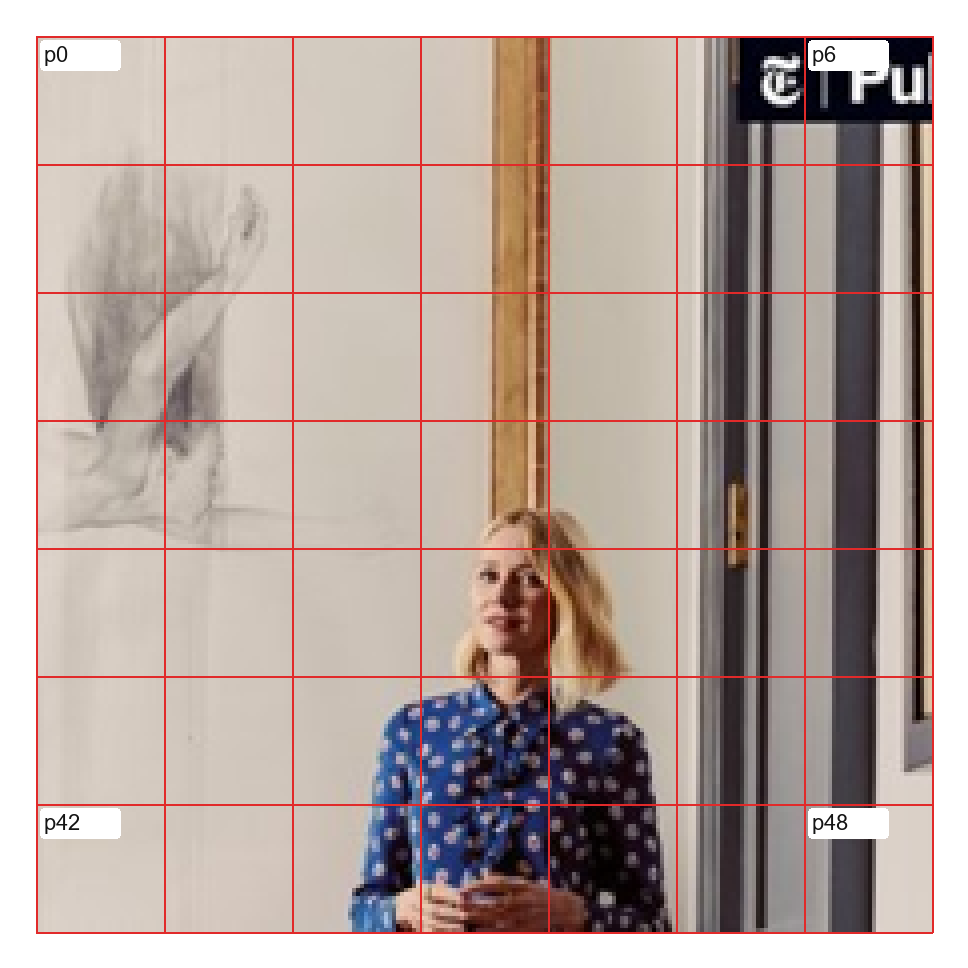
\includegraphics[width=0.55\linewidth]{figs/patch_grid.png}
\caption{预处理后的实际样本与 $7\times7$ 图块网格}
\label{fig:patch-grid}
\end{figure}

\subsection{多头注意力}

对于宽度 $D=768$、头数 $H=12$，每个头的维度为 $d_h=64$，\studenthighlight{将 Q、K、V 的线性结果由 $[B,N,D]$ 正确变形为 $[B,H,N,d_h]$。}注意力计算为
\[
\operatorname{Attention}(Q,K,V)=\operatorname{softmax}\left(\frac{QK^{\mathsf T}}{\sqrt{d_h}}\right)V.
\]
\studenthighlight{合并各头后，输出投影同样使用存储权重的转置。这里的关键是只交换 K 的最后两个轴，不能错误地转置批次维或头维。}

具体地说，先以一次矩阵乘法得到 $[B,N,3D]$ 的 QKV 拼接结果，再切分为三个 $[B,N,D]$ 数组。对于每个 batch、每个 head，$QK^{\mathsf T}$ 的形状是 $[N,N]$，表示任意两个 token 的关联分数。softmax 在最后一维进行，因此每个查询 token 对全部键 token 的注意力系数之和为 1。加权 V 后的各头结果为 $[B,H,N,64]$，转置为 $[B,N,H,64]$ 并合并为 $[B,N,768]$。

\subsection{Transformer block 与输出}

\studenthighlight{每个 block 依次执行归一化、注意力、第一次残差、归一化、MLP 与第二次残差。}MLP 的中间维度为 3072，使用课程给定的精确 GELU。\studenthighlight{最终阶段选择第 0 行 CLS token；\texttt{visual.proj} 的检查点布局已经是 $[768,512]$，因此不再转置。最后调用给定的单位向量函数，保证每一行输出的平方范数为 1。}

两次残差连接的作用分别是保留注意力更新前的 token 信息，以及保留 MLP 更新前的 token 信息。相应计算可概括为
\[
R=X+\operatorname{MHA}(\operatorname{LN}_1(X)),\qquad
Y=R+\operatorname{MLP}(\operatorname{LN}_2(R)).
\]
这种写法也是数值调试时的分界点：若 \texttt{block0} 首次出现偏差，应依次检查第一层归一化、注意力 head 组织、输出投影、第一处残差、第二层归一化和 MLP。

\section{代码仓库与复现说明}

为便于保存实验代码、版本管理与结果复现，本实验相关代码已保存至 GitHub 仓库：
\studenthighlight{\url{https://github.com/pppc111/Reproduce-the-OpenCLIP-ViT-B-32-image}}。

仓库包含本人完成的 \studenthighlight{\texttt{image\_encoder.py}、带有运行与验证说明的 \texttt{README.md}、实验报告源文件 \texttt{project1\_numpy.tex} 与图表文件}，以及课程提供的测试图像和参考输出；复现时需将课程附件中的\texttt{weights/}、\texttt{assets/}、\texttt{helpers.py}、\texttt{runtime.py}和 \texttt{check.py} 放入同一项目目录，再执行：
\begin{verbatim}
python check.py --stage all
python run.py --output output_tokens.npz
\end{verbatim}


\studenthighlight{为满足代码可读性与复现要求，\texttt{image\_encoder.py} 的六组 TODO 均保留了输入/输出形状、张量轴顺序、权重转置和残差连接的行内注释；\texttt{README.md} 给出了依赖课程附件的边界、运行命令及逐阶段数值验证表}，能从 GitHub 链接直接核对本人实现、代码注释和复现步骤。

\section{数值验证结果}

\studenthighlight{使用提供的 \texttt{check.py} 与 \texttt{assets/reference\_outputs.npz} 逐阶段比对。内部 token 的允许误差为 $2\times10^{-4}$，最终输出的绝对误差阈值为 $2\times10^{-5}$。表\ref{tab:results} 显示所有阶段均通过。}

\begin{table}[H]
\centering
\small
\caption{与独立参考输出的数值对照}
\label{tab:results}
\begin{tabular}{l c r r c}
\toprule
阶段 & 形状 & 最大绝对误差 & 平均绝对误差 & 结论 \\
\midrule
预处理 & $(10,3,224,224)$ & $0$ & $0$ & PASS \\
图块 & $(2,49,3072)$ & $0$ & $0$ & PASS \\
输入 token & $(2,50,768)$ & $7.153\times10^{-6}$ & $2.597\times10^{-7}$ & PASS \\
第 0 个 block & $(2,50,768)$ & $7.540\times10^{-6}$ & $2.455\times10^{-7}$ & PASS \\
最终 token & $(2,50,768)$ & $4.196\times10^{-5}$ & $2.438\times10^{-6}$ & PASS \\
输出 token & $(10,512)$ & $7.302\times10^{-7}$ & $8.244\times10^{-8}$ & PASS \\
批处理重排/重复 & $(3,512)$ & $4.992\times10^{-7}$ & $7.769\times10^{-8}$ & PASS \\
\bottomrule
\end{tabular}
\end{table}

\studenthighlight{图块阶段的零误差说明图块顺序与 C--H--W 内部展开顺序正确。误差在 12 层累计后仍远低于内部 token 容差；最终的投影与归一化将最大误差控制在输出阈值的约 $3.7\%$。}

图\ref{fig:errors} 将非零阶段的最大绝对误差置于对数坐标中。最终 token 的误差最大，但仍低于内部 token 容差 $2\times10^{-4}$；输出和批处理误差则明显低于 $2\times10^{-5}$ 的输出阈值。图块和预处理阶段的误差为零，未在对数图中绘制。

\begin{figure}[H]
\centering
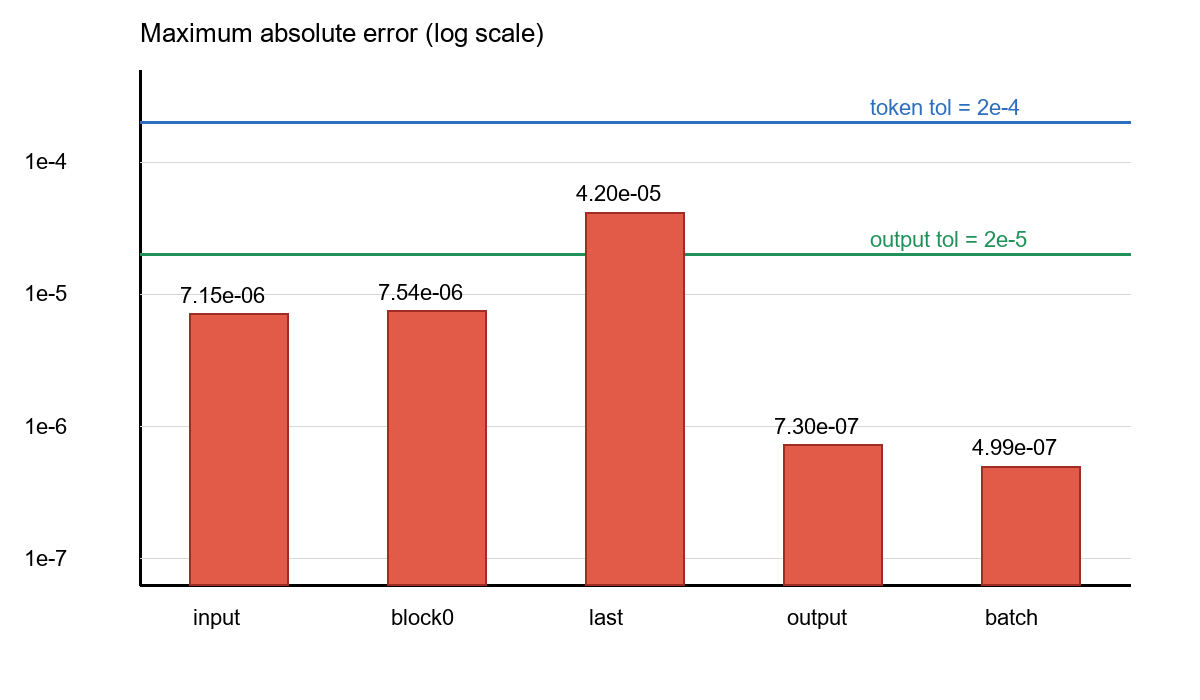
\includegraphics[width=0.7\linewidth]{figs/verification_errors.png}
\caption{各非零验证阶段的最大绝对误差及容差线（对数坐标）}
\label{fig:errors}
\end{figure}

\section{问题分析与改进}

\studenthighlight{调试中出现的问题都集中在形状与轴序}。典型bug为对已经按 [输入,输出]=$[768,512]$ 存储的 \texttt{visual.proj} 再做一次转置。二次转置直接引发形状冲突：$[768,512]$ 变成 $[512,768]$ 后与 $[B,768]$ 无法相乘，在 output 阶段报错。\studenthighlight{发现后删除了二次转置，使运行结果正确。}


实现中可做可读性改进。例如，可在 \texttt{patchify} 开头一次性解包 \texttt{B, C, H, W = images.shape}，避免重复访问形状属性，并在矩阵运算符两侧统一添加空格，在合并多头时把$B$、$H$、$N$、$d_h $在赋值处统一命名。


\section{个人贡献与工具使用说明}

\studenthighlight{本人独立完成\texttt{image\_encoder.py} 中六组实现与调试，具体包括图块构造、多头注意力、Transformer block、token 嵌入和最终输出，并使用课程提供的检查程序和参考数组逐阶段验证。}过程中使用的外部协助为：借助辅助工具阅读课程 \texttt{README} 与课件对照表、核对检查点中各张量的名称与形状、依据报错堆栈定位上述 AttributeError，以及整理本报告的文字与表格。课程提供的 \texttt{check.py}、\texttt{helpers.py}、\texttt{preprocess\_image.py}、权重文件与参考数组属于课程材料，不属于本人实现。代码的最终正确性以课程提供的独立参考输出为准。

\newpage

% ============================================================
% 批阅与成绩评定页
% ============================================================

% 绘制正文外框（包含批阅区域）
\begin{tikzpicture}[remember picture, overlay]
  \draw[thick] 
    ($(current page.north west)+(2cm,-3cm)$) 
    rectangle 
    ($(current page.south east)+(-2cm,3.5cm)$);
\end{tikzpicture}

\vspace{1cm}

% 批阅区
\noindent \textbf{指导教师批阅意见：}
\vspace{6cm}
\hfill

\vspace{1cm}

\noindent \textbf{成绩评定：}
\vspace{2cm}
\hfill

\vspace{1cm}

\begin{flushright}
\textbf{指导教师签字：}\quad\quad\quad\quad\quad\\[0.5cm]
\textbf{年}\quad\quad \textbf{月}\quad\quad \textbf{日}\quad
\end{flushright}

\vspace{1cm}

% 备注部分
\noindent \textbf{备注：}

% 框外的注释
\begin{tikzpicture}[remember picture, overlay]
  \node[
    anchor=north west,
    inner sep=0pt,
    text width=\dimexpr\paperwidth-4cm\relax
  ] at ($(current page.south west)+(2cm,3.1cm)$) {
    \begin{minipage}{\dimexpr\paperwidth-4cm\relax}
      \small
      \noindent
      \textbf{注：}\;1、报告内的项目或内容设置，可根据实际情况加以调整和补充。\\[0.2cm]
      \phantom{\textbf{注：}\;}2、教师批改学生实验报告时间应在学生提交实验报告时间后 10 日内。
    \end{minipage}
  };
\end{tikzpicture}

% ============================================================
%                      文档结束
% ============================================================

\end{document}
